\section{Conclusion}
\label{sec:conclusion}
In this paper, we present a gaze-aware neural scene representation and view synthesis method tailored for future portable virtual reality viewing experiences. Specifically, we overcome the limitations of existing neural rendering approaches for high performance, resolution, and fidelity. Our network individually synthesizes foveal, mid-, and far-periphery retinal images, which are then blended to form a wide field-of-view image matching retinal acuity. This is achieved via adapting the neural network model to the foveated visual acuity and stereopsis. 
Comparing with traditional rendering, our method requires less than $1\%$ data storage yet delivering identically high perceptual quality.
Comparing with alternative neural view synthesis approaches, our method creates significantly faster and higher fidelity viewing for high resolution, high FoV, and stereo VR head-mounted-displays.
%The experiments with user studies, objective measurements, and intra-system analysis show our significant effectiveness of delivering perceptually identical visual contents in real-time.
 
\paragraph{Limitations and future work}
While our method achieves unprecedented performance compared to existing approaches, it suffers from a few limitations. Our multi-spherical representation introduces higher quality when the VR camera is within the first sphere. As shown in \Cref{fig:large_translation}, when the virtual camera translates largely within a highly occluded scene, our method still synthesizes the accurate views but with declined foveal image quality. This is due to the accumulated error of the concentric spherical representation (\Cref{eq:imageError}).
Multiscale coordinates and networks that consider various level-of-details of the 3D space have shown their effectiveness of interpolating geometries \cite{winkler2010multi}. Developing a multiscale network that synthesizes the image from global to local level-of-details would be an interesting direction for future work, extending the applicability of our method to large-scale scenes with strong occlusions.
\begin{figure}[!ht]
    \centering
    % \subfloat[small translation]{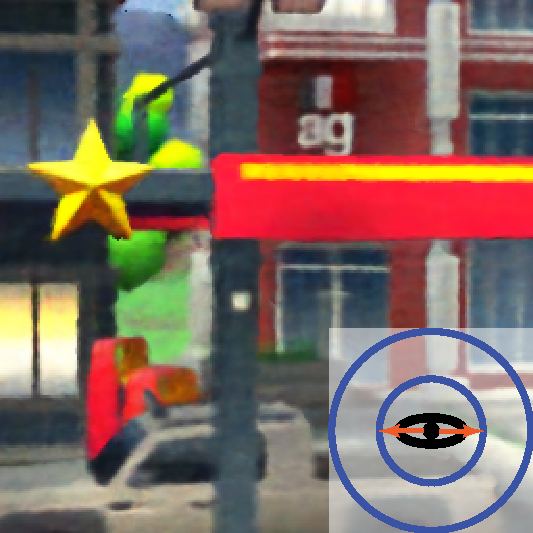
\includegraphics[width=0.47\linewidth]{TOG/figs/large_tran/2_gas_0.3.pdf}\label{fig:large_translation:small}}\hspace{1em} % or 2_gas_0.3.png
    \subfloat[small translation]{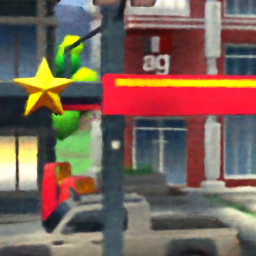
\includegraphics[width=0.47\linewidth]{TOG/figs/large_tran/2_gas_0.3.png}\label{fig:large_translation:small}}\hspace{1em}
    % \subfloat[large translation]{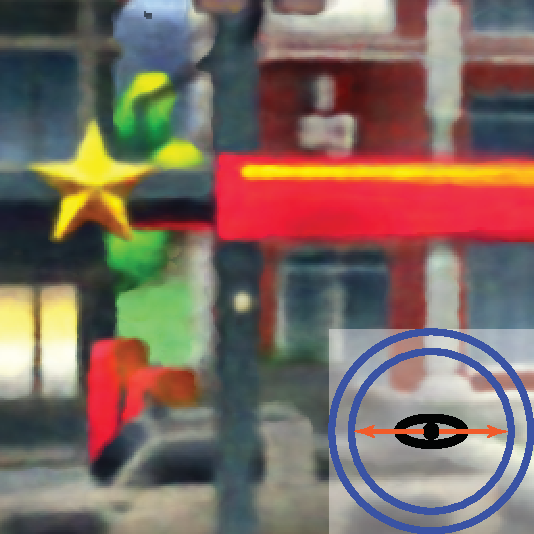
\includegraphics[width=0.47\linewidth]{TOG/figs/large_tran/2_gas_0.9.pdf}\label{fig:large_translation:large}} % or 2_gas_0.9.png
    \subfloat[large translation]{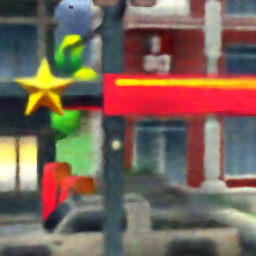
\includegraphics[width=0.47\linewidth]{TOG/figs/large_tran/2_gas_0.9.png}\label{fig:large_translation:large}}
    \Caption{Comparing foveal quality with regards to translation range. }
    {%
    Using our method, \subref{fig:large_translation:small} shows a fovea image \dnc{from training dataset} with a small-scale translation box (0.3m); \subref{fig:large_translation:large} shows a fovea image with a large-scale translation box (0.9m).
    }
    \label{fig:large_translation}
\end{figure}

Currently, we sample the scene fully based on eccentricity, considering acuity and stereopsis. However, we envision that fine-grained visual sensitivity analysis, such as luminance \cite{Tursun:2019:LCA} or depth \cite{Sun:20:OE}, would provide more insights on achieving even higher quality and/or faster performance. Also, our multi-spherical representation is specialized to the scene for optimal quality. Thus, our network is trained per-scene. Exploring potential means of generalized representation may further reduce storage.

For simplicity, the spatial-temporal joint optimization in \Cref{sec:method:optimization} connects the output precision and latency to the number of the spheres ($\sphereNum$) but not their radii $\mathbf{\sphereRadius}$. This is due to the significant amount of training with parameter sampling. Incorporating the parameters into a single training process may significantly reduce the time consumption for the optimization. With the adaptive training process, a content-aware distribution (i.e., $\mathbf{\sphereRadius}$) of the spheres would further improve the synthesis quality and performance.
%\qisun{note to myself: Right now we use did not optimize for radii but only number of spheres}

\zh{shall we end with non-limitation sentences?}\qisun{yep, future work is positive than limitations.;)}